% This file provides examples of some useful macros for typesetting
% dissertations.  None of the macros defined here are necessary beyond
% for the template documentation, so feel free to change, remove, and add
% your own definitions.
%
% We recommend that you define macros to separate the semantics
% of the things you write from how they are presented.  For example,
% you'll see definitions below for a macro \file{}: by using
% \file{} consistently in the text, we can change how filenames
% are typeset simply by changing the definition of \file{} in
% this file.
% 
%% The following is a directive for TeXShop to indicate the main file
%%!TEX root = diss.tex

\newcommand{\NA}{\textsc{n/a}}	% for "not applicable"
\newcommand{\eg}{e.g.,\ }	% proper form of examples (\eg a, b, c)
\newcommand{\ie}{i.e.,\ }	% proper form for that is (\ie a, b, c)
\newcommand{\etal}{\emph{et al}}

% Some useful macros for typesetting terms.
\newcommand{\file}[1]{\texttt{#1}}
\newcommand{\class}[1]{\texttt{#1}}
\newcommand{\latexpackage}[1]{\href{http://www.ctan.org/macros/latex/contrib/#1}{\texttt{#1}}}
\newcommand{\latexmiscpackage}[1]{\href{http://www.ctan.org/macros/latex/contrib/misc/#1.sty}{\texttt{#1}}}
\newcommand{\env}[1]{\texttt{#1}}
\newcommand{\BibTeX}{Bib\TeX}

% Define a command \doi{} to typeset a digital object identifier (DOI).
% Note: if the following definition raise an error, then you likely
% have an ancient version of url.sty.  Either find a more recent version
% (3.1 or later work fine) and simply copy it into this directory,  or
% comment out the following two lines and uncomment the third.
\DeclareUrlCommand\DOI{}
\newcommand{\doi}[1]{\href{http://dx.doi.org/#1}{\DOI{doi:#1}}}
%\newcommand{\doi}[1]{\href{http://dx.doi.org/#1}{doi:#1}}

% Useful macro to reference an online document with a hyperlink
% as well with the URL explicitly listed in a footnote
% #1: the URL
% #2: the anchoring text
\newcommand{\webref}[2]{\href{#1}{#2}\footnote{\url{#1}}}

% epigraph is a nice environment for typesetting quotations
\makeatletter
\newenvironment{epigraph}{%
	\begin{flushright}
	\begin{minipage}{\columnwidth-0.75in}
	\begin{flushright}
	\@ifundefined{singlespacing}{}{\singlespacing}%
    }{
	\end{flushright}
	\end{minipage}
	\end{flushright}}
\makeatother

% \FIXME{} is a useful macro for noting things needing to be changed.
% The following definition will also output a warning to the console
\newcommand{\FIXME}[1]{\typeout{**FIXME** #1}\textbf{[FIXME: #1]}}

% END

% Modified \textcircled solution
\newcommand*\circled[1]{\raisebox{.5pt}{\textcircled{\raisebox{-.9pt} {#1}}}}


% https://tex.stackexchange.com/questions/172475/how-can-i-define-a-custom-tcolorbox-environment-with-color-as-a-parameter
\definecolor{mycolor}{rgb}{0.122, 0.435, 0.698}
\definecolor{blackcolor}{rgb}{0, 0, 0}
\definecolor{lightgray}{gray}{0.9}

\definecolor{error}{HTML}{FFD5D4}
\definecolor{relevant}{HTML}{E0F8C7}
\definecolor{steelblue}{RGB}{0, 0, 152}
\definecolor{royalblue}{RGB}{65,105,225}
\definecolor{rufous}{rgb}{0.66, 0.11, 0.03}

\newmdenv[innerlinewidth=0.5pt, roundcorner=1pt,linecolor=blackcolor,innerleftmargin=4pt,
innerrightmargin=4pt,innertopmargin=4pt,innerbottommargin=4pt]{mybox}



% Author's comments
\newcommand{\gm}[1]{\textcolor{orange}{{\textit{GM: #1}}}}
\newcommand{\gcm}[1]{\textcolor{orange}{{\textit{GM: #1}}}}
\newcommand{\art}[1]{\textcolor{red}{{\textit{AM: #1}}}}


% Bullet while on draft mode
\newcommand{\blt}{\smallskip \textbullet ~}


% Counters
\newcounter{rq}

\newcommand{\RQ}[1]{\textit{RQ\the\numexpr\arabic{rq}\relax}}


\newcommand{\red}[1]{\textcolor{red}{#1}}
\newcommand{\rev}[1]{\textcolor{steelblue}{#1}}
\newcommand{\orange}[1]{\textcolor{orange}{#1}}


\definecolor{Brow}{HTML}{792500}


% Highlight package, default colour set to ligthgray
\sethlcolor{lightgray}

% https://tex.stackexchange.com/questions/50792/a-better-pm-symbol
\makeatletter
\newcommand{\mypm}{\mathbin{\mathpalette\@mypm\relax}}
\newcommand{\@mypm}[2]{\ooalign{%
  \raisebox{.1\height}{$#1+$}\cr
  \smash{\raisebox{-.6\height}{$#1-$}}\cr}}
\makeatother


% https://tex.stackexchange.com/questions/22798/nice-looking-empty-set
\let\oldemptyset\emptyset
\let\emptyset\varnothing

\usepackage{pifont}% http://ctan.org/pkg/pifont
\newcommand{\cmark}{\ding{51}}%
\newcommand{\xmark}{\ding{55}}%

\newtcolorbox{bluequote}{enhanced,
  boxrule=0pt,
  frame hidden,
  borderline west={4pt}{0pt}{lightgray},
  colback=white,
  sharp corners,
  right=0pt, 
  top=0pt, 
  bottom=0pt}


% https://tex.stackexchange.com/questions/69148/how-to-insert-title-in-mdframed
\newenvironment{frameEnv}[1]
  {\mdfsetup{
    frametitle={\colorbox{white}{\space#1\space}},
    frametitlefont=\ttfamily,
	  innertopmargin=1pt,
    frametitleaboveskip=-\ht\strutbox,
    frametitlealignment=\center
    }
  \begin{mdframed}%
  }
  {\end{mdframed}}


\newtcolorbox{keyobs}[1][]{
  breakable,  
  colback=white,
  colbacktitle=white,
  coltitle=black,
  fonttitle=\bfseries,
  bottomrule=0pt,
  toprule=0pt,
  leftrule=3pt,
  rightrule=0pt,
  titlerule=0pt,
  arc=0pt,
  outer arc=0pt,
  colframe=black,
}




% example of minipage

% \begin{figure}
%   \centering
%   \begin{minipage}{.5\textwidth}
%       \centering
%       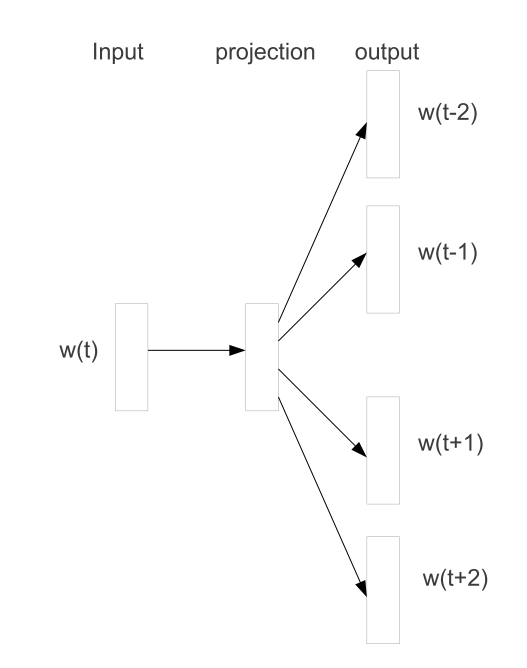
\includegraphics[width=0.5\linewidth, height=0.2\textheight]{fig/cp5/skip-gram-architecture}
%       \caption{The Skip-gram model architecture~\cite{Mikolov2013}}
%       \label{fig:skip-gram}
%   \end{minipage}%
%   \begin{minipage}{0.5\textwidth}
%       \centering
%       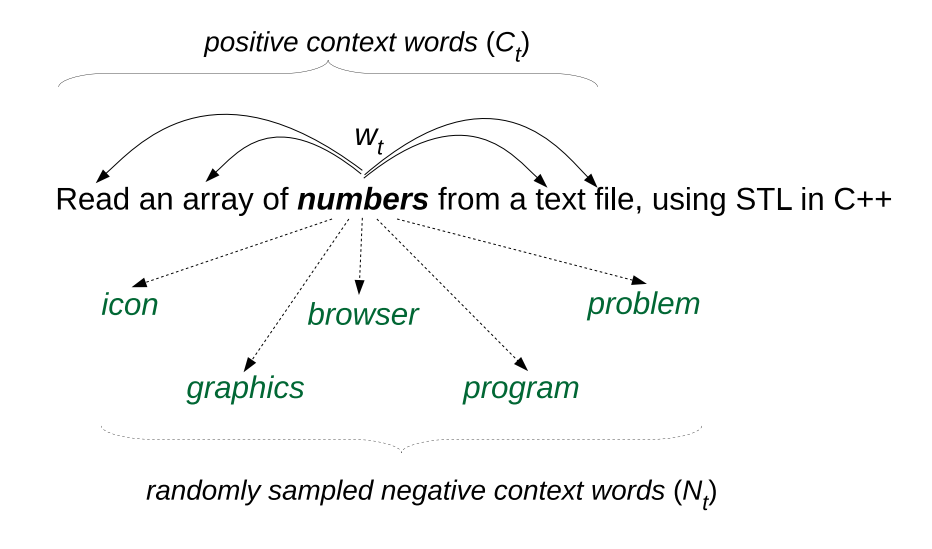
\includegraphics[width=\linewidth, height=0.2\textheight]{fig/cp5/ye-skip-gram-example}
%       \caption{Positive and negative training examples~\cite{Ye2016}}
%       \label{fig:skip-gram-example}
%   \end{minipage}
% \end{figure}

